% chapters/02_marco_teorico.tex
\chapter{Fundamentos teóricos de la optimización basada en modelos sustitutos}
\label{chap:marco_teorico}

Muchos problemas reales de optimización en ingeniería y ciencia de datos pueden formularse mediante una función objetivo $f : X \to \mathbb{R}$ cuyo valor solo puede obtenerse evaluando un procedimiento externo, como una simulación numérica compleja o un experimento físico. En este contexto, se dice que la función es de \textit{caja negra} cuando, a efectos prácticos, no se dispone de una expresión analítica manejable de $f$, ni de derivadas, ni de propiedades estructurales que permitan aplicar directamente métodos clásicos de optimización. En otras palabras, la función solo puede consultarse en puntos concretos del dominio y devolver una salida asociada a cada entrada.

Además, en muchos de estos problemas cada evaluación de $f(x)$ tiene un coste elevado, ya sea en tiempo de cómputo o uso de recursos. Así, la dificultad no reside únicamente en que la función sea desconocida internamente, sino también en que solo puede evaluarse un número reducido de veces.


\vspace{0.3cm}
Con el fin de formalizar este problema, introducimos un espacio de búsqueda continuo $\mathcal{X}\subset\mathbb{R}^{d}$ que contiene todas las posibles configuraciones de las variables de entrada, junto con una función objetivo $f:\mathcal{X}\to\mathbb{R}$ que modela el comportamiento del sistema. El propósito de la \emph{optimización global} es encontrar un minimizador global
\[
\bm{x}^{\star} \in \arg\min_{\bm{x}\in\mathcal{X}} f(\bm{x}).
\]
Nuestra hipótesis de trabajo es que el coste $c(\bm{x})$ de evaluar la función objetivo es elevado. En consecuencia, el número de evaluaciones que pueden realizarse queda limitado por un presupuesto máximo $B$, de modo que solo se dispone de un conjunto reducido de observaciones:
\[
\mathcal{D}_n = \{(\bm{x}_i, y_i)\}_{i=1}^{n}, \qquad n \leq B,
\]
donde $y_i$ representa el valor observado al evaluar la función en el punto $\bm{x}_i$.

Incluso en aquellos casos en los que el coste individual de evaluación fuera asumible, la búsqueda exhaustiva seguiría siendo inviable cuando la dimensión del espacio $\mathcal{X}$ es elevada. En efecto, el número de puntos necesarios para explorar el dominio con una densidad comparable crece exponencialmente con la dimensión, fenómeno conocido como \emph{maldición de la dimensionalidad}. Por tanto, la dificultad del problema no proviene únicamente del coste por evaluación, sino también del tamaño efectivo del espacio de búsqueda. 

Además del coste, en muchos problemas las evaluaciones están afectadas por \emph{ruido}. En experimentos físicos, el ruido proviene de errores de medida, variabilidad del entorno o diferencias entre réplicas. En simulaciones complejas, puede aparecer \emph{ruido numérico} debido a múltiples causas como fenómenos estocásticos internos. Una forma estándar de modelar esta situación es asumir que la observación es una perturbación de la función subyacente:

\[
y_i = f(\bm{x}_i) + \varepsilon_i, 
\qquad 
\mathbb{E}[\varepsilon_i]=0,
\qquad 
\mathrm{Var}(\varepsilon_i)=\sigma_\varepsilon^2.
\]
Estas dos restricciones (presupuesto limitado y/o ruido) hacen que muchos optimizadores clásicos resulten poco adecuados: los métodos basados en gradientes requieren derivadas (normalmente no disponibles en caja negra) y pueden ser inestables bajo ruido. En consecuencia, el problema se transforma en una búsqueda bajo escasez de datos: con pocas evaluaciones debemos (i) aproximar $f$ lo suficiente como para guiar la búsqueda y (ii) decidir adaptativamente dónde invertir las siguientes evaluaciones para mejorar la solución global.

Esta motivación conduce de forma natural al enfoque de \emph{optimización basada en modelos sustitutos} (SBO) que consiste en construir un modelo estadístico $\hat{f}$ a partir de $\mathcal{D}_n$ y emplearlo para proponer nuevas evaluaciones, reduciendo de manera drástica el número de consultas directas a la función costosa \cite{forrester2008engineering,jiang2020surrogate}. En las siguientes secciones se introducen estos modelos y cómo se integran.

\section{Modelos sustitutos: definición y taxonomía}
\label{sec:surrogates_def_tax}

En este contexto de optimización con evaluaciones costosas, un \emph{modelo sustituto}
(o \emph{metamodelo}) se define como una aproximación $\hat{f}$ aprendida a partir de un
conjunto finito de observaciones
$
\mathcal{D}_n=\{(\bm{x}_i,y_i)\}_{i=1}^n,$
con el objetivo de emular la respuesta del sistema real a un coste computacional muy
inferior al de evaluar directamente la función objetivo original \cite{forrester2008engineering,jiang2020surrogate}.
\newline
Un modelo sustituto puede emplearse con dos fines principales:
\begin{enumerate}
  \item \textbf{Predicción rápida y análisis del espacio de diseño.} Una vez entrenado,
  $\hat{f}$ permite evaluar muchas configuraciones de entrada para comprender tendencias,
  analizar sensibilidad o explorar regiones de interés sin ejecutar el sistema costoso.
  \item \textbf{Optimización con presupuesto limitado.} En SBO,
  el sustituto se utiliza para guiar la selección de nuevas evaluaciones del sistema real,
  reduciendo el número de ejecuciones costosas necesarias para aproximarse a la solución
  óptima \cite{jiang2020surrogate}.
\end{enumerate}

\medskip
\noindent Existe gran variedad de modelos que pueden actuar como sustitutos. Una taxonomía orientada a la práctica, es la siguiente:
\begin{itemize}
  \item \textbf{Según la naturaleza de la predicción:}
  \begin{description}
    \item [Deterministas] Producen una predicción puntual $\hat{f}(\bm{x})$.
    \item [Probabilísticos] Cuantifican incertidumbre (p.\,ej. mediante una
    distribución predictiva). Esta distinción es relevante cuando se quieren criterios de
    muestreo adaptativo basados en exploración/explotación \cite{forrester2008engineering,jiang2020surrogate}.
  \end{description}

  \item \textbf{Según la flexibilidad del modelo:}
  \begin{description}
    \item [Paramétricos] (p.\,ej. regresiones polinómicas). Simples e interpretables, pero
    potencialmente rígidos si la respuesta presenta multimodalidad o alta no linealidad.
    \item [No paramétricos o de alta flexibilidad] (p.\,ej. métodos kernel, árboles, \emph{ensembles}).
    Capaces de capturar respuestas complejas, a costa de más parámetros y riesgo de sobreajuste
    con pocos datos \cite{forrester2008engineering}.
  \end{description}

  \item \textbf{Según cómo se integra con la optimización:}
  \begin{description}
    \item[Offline] Se entrena una única vez con $\mathcal{D}_n$ y se utiliza para proponer
    candidatos (útil cuando obtener nuevas evaluaciones es inviable en el corto plazo).
    \item[Secuencial/online] El sustituto se actualiza iterativamente añadiendo nuevas
    evaluaciones seleccionadas de forma informada (infill/adaptive sampling), hasta agotar presupuesto
    o alcanzar un criterio de parada \cite{forrester2008engineering,jiang2020surrogate}.
  \end{description}
\end{itemize}

\medskip
\noindent A pesar de la diversidad de modelos, el proceso general de modelado sustituto sigue un flujo de trabajo
estándar:
\begin{enumerate}
  \item \textbf{Definir variables y dominio.} Se establecen las variables de decisión (entradas)
  y sus rangos, fijando el dominio $\mathcal{X}$.
  \item \textbf{Muestreo inicial (DoE).} Se selecciona un conjunto inicial de puntos
  $\{\bm{x}_i\}_{i=1}^n$ que cubra el espacio de forma razonablemente uniforme. En problemas
  continuos es habitual usar muestreos \emph{space-filling}, como Latin Hypercube Sampling (LHS) o SOBOL
  \cite{forrester2008engineering}.
  \item \textbf{Evaluación del sistema real.} Se calculan las salidas $y_i$ con el sistema real
  y se construye el dataset inicial $\mathcal{D}_n$.
  \item \textbf{Ajuste y validación del sustituto.} Se elige una familia de modelos, se estiman sus
  parámetros y se evalúa su calidad predictiva con prácticas estándar (p.\,ej. validación cruzada),
  teniendo presente compromisos entre complejidad y robustez \cite{forrester2008engineering}.
  \item \textbf{Refinamiento secuencial: muestreo adaptativo o proceso de \emph{infill}}.
  Cuando el presupuesto lo permite, se añaden nuevos puntos (\emph{infill points}) seleccionados
  por un criterio que prioriza:
  (i) regiones donde el modelo es probablemente inexacto (exploración), y/o
  (ii) regiones prometedoras respecto al óptimo (explotación). Este ciclo se repite hasta alcanzar
  un criterio de parada (en base a presupuesto máximo, mejora marginal, o precisión objetivo) \cite{forrester2008engineering,jiang2020surrogate}.
\end{enumerate}

\medskip
\noindent En este TFG, los modelos sustitutos se emplean principalmente con fines de optimización
bajo presupuesto limitado, sin perder su utilidad como herramienta de análisis e
interpretación del problema. Esta idea se estudiará en dos escenarios complementarios:
un conjunto de \emph{benchmarks}, donde la función objetivo puede evaluarse de forma
controlada para analizar el ciclo secuencial completo (pasando de $n=0$ o $n$ con muestreo inicial, a $B$ muestras), y un \emph{caso real}, donde el modelo
se entrenará con los datos disponibles para evaluar su rendimiento y proponer
configuraciones candidatas $\bm{x}^\star$ para una posible validación futura.
% =========================================================
% 2.3 El Proceso Gaussiano (GP)
% =========================================================

\section{El Proceso Gaussiano como modelo sustituto}
\label{sec:gp_surrogate}


Siguiendo principalmente a Rasmussen y Williams \cite{rasmussen2006gpml}, en esta
subsección se introduce el GP como modelo bayesiano de regresión no
paramétrica. Su interés en el contexto de los modelos sustitutos probabilísticos reside en
que, además de proporcionar una predicción media, ofrece una cuantificación analítica de la
incertidumbre, esencial en optimización bayesiana (BO). Para ello, se presentará primero la
definición del GP como distribución sobre funciones y, después, su interpretación a partir de
la regresión lineal bayesiana en espacio de características. La
Figura~\ref{fig:prior_vs_posterior} ilustra esta idea mostrando el paso de una distribución
prior sobre funciones a una distribución posterior tras observar datos.

\begin{figure}[htbp]
    \centering
    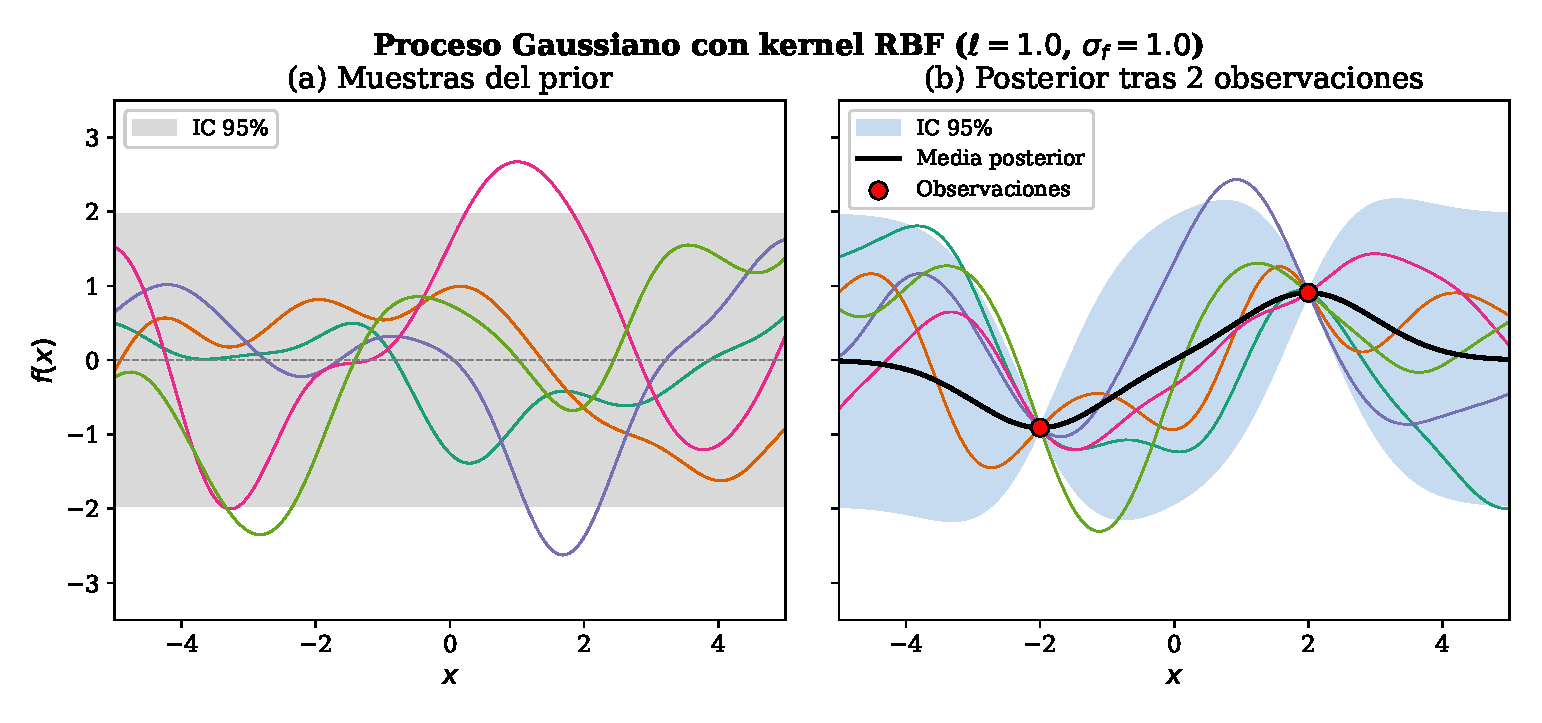
\includegraphics[width=0.8\textwidth]{assets/fig_gp_prior_posterior.eps}
    \caption[Prior y posterior de un GP]{(a) Muestras de funciones generadas por el prior del GP. (b) Distribución posterior tras condicionar en dos observaciones; la línea negra representa la media predictiva y la banda sombreada el intervalo predictivo del 95 \%.}
    \label{fig:prior_vs_posterior}
\end{figure}

\FloatBarrier

\subsection{Definición y consistencia}
\label{subsec:gp_definicion_consistencia}

Formalmente, un GP es un proceso estocástico definido sobre el espacio de entrada
$\mathcal{X}$ tal que, para cualquier conjunto finito de puntos $X=\{x_1,\dots,x_n\}\subset\mathcal{X}$,
el vector de valores de la función
\[
\mathbf{f}_X = \bigl(f(x_1),\dots,f(x_n)\bigr)^\top
\]
sigue una distribución normal multivariante. En consecuencia, existe una función de media
$m:\mathcal{X}\to\mathbb{R}$ y una función de covarianza $k:\mathcal{X}\times\mathcal{X}\to\mathbb{R}$ tales que
\[
\mathbf{f}_X \sim \mathcal{N}\!\bigl(\mathbf{m}_X,\mathbf{K}_{XX}\bigr),
\]
donde
\begin{equation}
\label{eq:gp_media_matriz_cov}
\mathbf{m}_X =
\begin{bmatrix}
m(x_1)\\
\vdots\\
m(x_n)
\end{bmatrix},
\qquad
(\mathbf{K}_{XX})_{ij}=k(x_i,x_j).
\end{equation}
De forma abreviada, se escribe
\[
f(x)\sim \mathcal{GP}\!\bigl(m(x),k(x,x')\bigr).
\]

\noindent La expresión anterior define el prior del GP sobre cualquier conjunto finito de
puntos. Por tanto, especificar un proceso gaussiano equivale a fijar dos objetos:
una función de media $m(x)$, que recoge la tendencia global esperada de la función,
y una función de covarianza $k(x,x')$, también llamada kernel, que determina cómo
se relacionan los valores de la función en distintos puntos del dominio.

La elección de la función de media forma parte de la especificación del prior. En general,
un GP no requiere media nula; sin embargo, una elección habitual es tomar $m(x)=0.$
Esta hipótesis resulta razonable cuando no se dispone de información previa clara
sobre una tendencia determinista global, ya que permite delegar la mayor parte de
la estructura del modelo en la función de covarianza. Además, aparece de forma
natural si se parte de un modelo lineal bayesiano centrado,
\[
f(x)=\phi(x)^\top w,
\qquad
w\sim\mathcal{N}(0,\Sigma_p),
\]
entonces la media inducida sobre la función satisface
\[
\mathbb{E}[f(x)] = \phi(x)^\top\mathbb{E}[w] = 0.
\]
Si existiera una tendencia conocida o relevante,
podría incorporarse mediante una función de media no nula o mediante funciones base
explícitas.

\medskip
\noindent Una vez fijada la media, el segundo elemento necesario para definir el prior es la
función de covarianza \(k(x,x')\), que induce la matriz de covarianza
\(\mathbf{K}_{XX}\), definida en la Ecuación~\eqref{eq:gp_media_matriz_cov}, que debe ser simétrica y semidefinida positiva para representar una covarianza válida. Intuitivamente, el kernel codifica las hipótesis a priori sobre la regularidad, suavidad y escala de variación de la función desconocida.

Además de definir media y covarianza, las distribuciones gaussianas asociadas a
distintos subconjuntos finitos del dominio deben ser coherentes entre sí. Esta
coherencia se obtiene gracias a una propiedad fundamental de la distribución
gaussiana multivariante: la consistencia bajo marginalización.

\begin{proposition}[Marginalización de una gaussiana multivariante]
\label{prop:marginalizacion_gaussiana}

Sea
\[
\begin{bmatrix}
\mathbf{f}_A\\
\mathbf{f}_B
\end{bmatrix}
\sim
\mathcal{N}\!\left(
\begin{bmatrix}
\boldsymbol{\mu}_A\\
\boldsymbol{\mu}_B
\end{bmatrix},
\begin{bmatrix}
\Sigma_{AA} & \Sigma_{AB}\\
\Sigma_{BA} & \Sigma_{BB}
\end{bmatrix}
\right),
\]
donde $\mathbf{f}_A$ y $\mathbf{f}_B$ son dos subvectores del vector gaussiano conjunto.
Entonces, la distribución marginal de $\mathbf{f}_A$ viene dada por

\[
\mathbf{f}_A \sim \mathcal{N}(\boldsymbol{\mu}_A,\Sigma_{AA}).
\]
\end{proposition}
En esta partición por bloques, $\Sigma_{AA}$ es la submatriz de covarianza asociada
exclusivamente a las componentes de $\mathbf{f}_A$, mientras que $\Sigma_{AB}$ y
$\Sigma_{BA}$ recogen las covarianzas cruzadas entre $\mathbf{f}_A$ y $\mathbf{f}_B$.

Esta propiedad garantiza que, aunque el GP esté definido sobre un dominio
potencialmente infinito, la inferencia puede realizarse de forma exacta utilizando únicamente
un número finito de puntos. En particular, basta con considerar la distribución conjunta de
los valores observados y, en su caso, de los puntos de predicción, ya que cualquier
subconjunto de variables del proceso sigue teniendo una distribución gaussiana coherente con
la especificación global.

La definición anterior introduce al GP directamente en el espacio de funciones (\emph{function-space view}): se especifica
un prior mediante su media y su función de covarianza, y la consistencia por marginalización
garantiza la coherencia de todas las distribuciones finitas inducidas. Sin embargo, esta
formulación todavía no muestra con claridad de dónde surge el kernel ni cómo debe
interpretarse el aprendizaje del modelo. Para ello, resulta útil volver a una construcción más
familiar: la regresión lineal bayesiana en un espacio de características, desde la cual el GP
aparece al marginalizar los pesos.

\subsection{Del espacio de pesos al espacio de funciones}

Para comprender con mayor precisión el origen del kernel y el significado del aprendizaje en
un GP, resulta útil partir de la regresión lineal bayesiana clásica y observar
cómo se transita desde un modelo definido por parámetros explícitos (\emph{weight-space view}) hacia una formulación
basada únicamente en covarianzas entre datos (\emph{function-space view}). Consideremos una función latente modelada como una combinación lineal de funciones base:
\[
f(\bm{x}) = \bm{\phi}(\bm{x})^\top \bm{w},
\]
donde \(\bm{\phi}(\bm{x})\in\mathbb{R}^N\) representa el vector de características asociado a
la entrada \(\bm{x}\) y \(\bm{w}\in\mathbb{R}^N\) es el vector de pesos. En lugar de asumir que
existe un único valor verdadero y desconocido de \(\bm{w}\) (enfoque frecuentista), el enfoque bayesiano introduce
incertidumbre sobre dichos parámetros mediante un prior gaussiano:
\(
\bm{w}\sim\mathcal{N}(\bm{0},\bm{\Sigma}_p).
\) Las observaciones no se consideran iguales a la función latente, sino realizaciones ruidosas
de la misma. Para cada dato observado se asume
\[
y_i = f(\bm{x}_i)+\varepsilon_i,
\qquad
\varepsilon_i\sim\mathcal{N}(0,\sigma_n^2),
\]
con ruido gaussiano independiente e idénticamente distribuido. Si definimos
\(\bm{y}=[y_1,\dots,y_n]^\top\) y la matriz de diseño en el espacio de características como
\[
\bm{\Phi}=
\begin{bmatrix}
\bm{\phi}(\bm{x}_1) & \cdots & \bm{\phi}(\bm{x}_n)
\end{bmatrix}
\in\mathbb{R}^{N\times n},
\]
entonces el modelo probabilístico para las observaciones puede escribirse como
\[
\bm{y}\mid X,\bm{w}\sim\mathcal{N}(\bm{\Phi}^\top\bm{w},\sigma_n^2\bm{I}).
\]

En la vista en espacio de pesos, aprender a partir de los datos equivale a actualizar
de forma bayesiana la distribución sobre \(\bm{w}\). Aplicando la regla de Bayes,
\[
p(\bm{w}\mid X,\bm{y}) \propto p(\bm{y}\mid X,\bm{w})\,p(\bm{w}),
\]
y dado que tanto la verosimilitud como el prior son gaussianos, la posterior vuelve a ser
gaussiana. En concreto,
\[
p(\bm{w}\mid X,\bm{y})=
\mathcal{N}(\bar{\bm{w}},\bm{A}^{-1}),
\qquad
\bm{A}=\sigma_n^{-2}\bm{\Phi}\bm{\Phi}^\top+\bm{\Sigma}_p^{-1},
\qquad
\bar{\bm{w}}=\sigma_n^{-2}\bm{A}^{-1}\bm{\Phi}\bm{y}.
\]
Esta expresión resume qué significa aprender en la \emph{weight-space view}: los datos no
fijan un único vector de pesos, sino que actualizan la distribución de probabilidad sobre
ellos. La media posterior \(\bar{\bm{w}}\) representa la localización más plausible de los
pesos tras observar los datos, mientras que \(\bm{A}^{-1}\) cuantifica la incertidumbre
residual sobre dichos parámetros.

A partir de esta posterior puede obtenerse ya una distribución predictiva para un nuevo
punto \(\bm{x}_*\). En efecto, si
$
f_* = f(\bm{x}_*)=\bm{\phi}(\bm{x}_*)^\top \bm{w},
$
entonces la predictiva se obtiene marginalizando la incertidumbre sobre \(\bm{w}\):
\[
p(f_*\mid \bm{x}_*,X,\bm{y})
=
\int p(f_*\mid \bm{x}_*,\bm{w})\,p(\bm{w}\mid X,\bm{y})\,d\bm{w}.
\]
Como \(f_*\) es una transformación lineal de una variable gaussiana, esta distribución es
también gaussiana:
\[
p(f_*\mid \bm{x}_*,X,\bm{y})
=
\mathcal{N}\!\Bigl(
\bm{\phi}(\bm{x}_*)^\top \bar{\bm{w}},
\;
\bm{\phi}(\bm{x}_*)^\top \bm{A}^{-1}\bm{\phi}(\bm{x}_*)
\Bigr).
\]

Esta formulación muestra de forma explícita cómo la incertidumbre sobre los pesos se
propaga a la predicción. Sin embargo, también revela una limitación: la
inferencia depende de \(\bm{A}^{-1}\), una matriz de tamaño \(N\times N\), donde \(N\) es la
dimensión del espacio de características. Si dicho espacio es muy grande o incluso infinito,
esta representación deja de ser operativa. El paso decisivo consiste entonces en reescribir el
modelo únicamente en términos de productos internos entre características.

De hecho, bajo el prior gaussiano sobre \(\bm{w}\), la función latente evaluada en cualquier
punto \(\bm{x}\) es también una variable aleatoria gaussiana, al ser combinación lineal de
variables gaussianas. Por tanto, para cualquier conjunto finito de entradas, la distribución
conjunta de los valores de la función queda completamente determinada por su media y su
covarianza. En particular,
\[
\mathbb{E}[f(\bm{x})]
=
\mathbb{E}[\bm{\phi}(\bm{x})^\top\bm{w}]
=
\bm{\phi}(\bm{x})^\top\mathbb{E}[\bm{w}]
=
0,
\]
y, para dos puntos arbitrarios \(\bm{x}\) y \(\bm{x}'\),
\[
\operatorname{cov}\bigl(f(\bm{x}),f(\bm{x}')\bigr)
=
\mathbb{E}\!\left[
\bm{\phi}(\bm{x})^\top \bm{w}\bm{w}^\top \bm{\phi}(\bm{x}')
\right]
=
\bm{\phi}(\bm{x})^\top \bm{\Sigma}_p \bm{\phi}(\bm{x}').
\]
La dependencia respecto a los pesos y a su covarianza puede agruparse en una única función definida sobre pares de
entradas:
$
k(\bm{x},\bm{x}')
=
\bm{\phi}(\bm{x})^\top \bm{\Sigma}_p \bm{\phi}(\bm{x}').
$
Así, la incertidumbre originalmente modelada sobre los parámetros \(\bm{w}\) se traslada a la
estructura de covarianza entre valores de la función.

Desde esta perspectiva, para cualquier conjunto finito
\(X=\{\bm{x}_1,\dots,\bm{x}_n\}\), el vector de valores latentes
$
\bm{f}_X =
\bigl(f(\bm{x}_1),\dots,f(\bm{x}_n)\bigr)^\top
$
puede obtenerse marginalizando los pesos:
\[
p(\bm{f}_X\mid X)
=
\int p(\bm{f}_X\mid X,\bm{w})\,p(\bm{w})\,d\bm{w}.
\]
Dado que \(\bm{f}_X=\bm{\Phi}^\top \bm{w}\) es una transformación lineal de una variable
gaussiana, su distribución marginal es también gaussiana, con
\[
\mathbb{E}[\bm{f}_X]=\bm{0},
\qquad
\operatorname{cov}(\bm{f}_X)=\bm{\Phi}^\top \bm{\Sigma}_p \bm{\Phi}=\bm{K},
\quad \text{con } K_{ij}=k(\bm{x}_i,\bm{x}_j).
\]
Por tanto,
\[
\bm{f}_X \sim \mathcal{N}(\bm{0}_X,\bm{K}_X).
\]
Es decir, al marginalizar los pesos se obtiene directamente una distribución gaussiana sobre
los valores de la función en cualquier conjunto finito de entradas. Esta es precisamente la
formulación del GP en el espacio de funciones: el modelo deja de expresarse
en términos explícitos de \(\bm{w}\) y pasa a quedar determinado únicamente por su función
de media y por su función de covarianza.

\paragraph{El truco del núcleo}
\label{subsec:truco_del_kernel}

Para conectar el truco del núcleo con su interpretación funcional, resulta útil recurrir
a la teoría de espacios de Hilbert con kernel reproductor. En esta parte se sigue la
presentación de los métodos kernel de Bishop \cite{bishop2006prml} y la interpretación
de RKHS y regularización de Hastie, Tibshirani y Friedman \cite{hastie2009elements}.
\vspace{0.3cm}

La expresión anterior
\(
k(\bm{x},\bm{x}')
=
\bm{\phi}(\bm{x})^\top \bm{\Sigma}_p \bm{\phi}(\bm{x}')
\)
muestra que la covarianza entre dos evaluaciones de la función no depende de los pesos
\(\bm{w}\) de forma explícita, sino únicamente de cómo se relacionan las entradas
\(\bm{x}\) y \(\bm{x}'\) en el espacio de características inducido por \(\bm{\phi}\) y ponderado
por \(\bm{\Sigma}_p\). Este es el punto en el que aparece el truco del núcleo.

Dado que \(\bm{\Sigma}_p\) es semidefinida positiva, puede escribirse en términos de una raíz
matricial \(\bm{\Sigma}_p^{1/2}\). Definiendo entonces un nuevo mapa de características
$
\bm{\psi}(\bm{x})=\bm{\Sigma}_p^{1/2}\bm{\phi}(\bm{x}),
$
la covarianza anterior puede reescribirse como
\[
k(\bm{x},\bm{x}')
=
\bm{\psi}(\bm{x})^\top \bm{\psi}(\bm{x}').
\]
Por tanto, el kernel puede interpretarse como un producto interno en un espacio de
características transformado. Esta observación tiene una consecuencia fundamental: si las
expresiones del modelo dependen únicamente de productos internos entre entradas
transformadas, entonces no es necesario construir ni manipular de forma explícita el vector
de características \(\bm{\phi}(\bm{x})\). Basta con disponer de una función
\(k(\bm{x},\bm{x}')\) que devuelva directamente ese producto interno.

En consecuencia, el modelo puede operar implícitamente en espacios de características de
dimensión muy alta, e incluso infinita, sin abandonar una formulación computable. En el
caso de los procesos gaussianos, esto significa que la inferencia y la predicción pueden
expresarse únicamente en términos de la matriz kernel \(\bm{K}\), cuyos elementos son
\(
K_{ij}=k(\bm{x}_i,\bm{x}_j).
\)
La complejidad algebraica deja así de depender de la construcción explícita del espacio de
características y se traslada al manejo de matrices de covarianza definidas sobre los datos
observados.

Desde un punto de vista conceptual, el truco del kernel no es solo una simplificación
computacional. También permite separar dos niveles de modelado: por un lado, la elección
de una función kernel \(k\), que codifica hipótesis a priori sobre suavidad, regularidad o
estructura de la función desconocida; por otro, la representación concreta en términos de
funciones base, que puede permanecer implícita. Esta reformulación justifica que, una vez introducido el GP desde la regresión lineal
bayesiana, el análisis posterior pueda desarrollarse enteramente en términos de funciones de
covarianza.

\paragraph{RKHS y teorema de representación.}
La interpretación anterior puede precisarse mediante el concepto de espacio de Hilbert con
kernel reproductor (\emph{Reproducing Kernel Hilbert Space}, RKHS). Dado un kernel
simétrico y semidefinido positivo \(k\), existe un espacio de Hilbert \(\mathcal{H}_k\) formado
por funciones \(f:\mathcal{X}\to\mathbb{R}\) en el que cada sección \(k(\cdot,\bm{x})\) pertenece al
espacio y satisface la propiedad reproductora:
\[
f(\bm{x})=\langle f,\;k(\cdot,\bm{x})\rangle_{\mathcal{H}_k}.
\]
Además, el propio kernel verifica
\[
k(\bm{x},\bm{x}')=
\langle k(\cdot,\bm{x}),\,k(\cdot,\bm{x}')\rangle_{\mathcal{H}_k}.
\]
Esta propiedad permite interpretar el kernel como un producto interno en un espacio de
características posiblemente de dimensión muy alta o infinita. En el espacio original
\(\mathcal{X}\), la relación entre las entradas y la salida puede ser no lineal; sin embargo,
mediante un levantamiento adecuado a un espacio funcional más rico, dicha relación puede
tratarse mediante operaciones lineales en ese nuevo espacio. En el marco de RKHS, este
levantamiento viene dado de forma canónica por
\(
\Phi_k(\bm{x})=k(\cdot,\bm{x}),
\)
de modo que
\[
k(\bm{x},\bm{x}')=
\langle \Phi_k(\bm{x}),\Phi_k(\bm{x}')\rangle_{\mathcal{H}_k}.
\]
Por tanto, el kernel no solo actúa como una función de covarianza o como un producto
interno implícito, sino también como el objeto que define la geometría del espacio funcional
en el que vive la solución.

Esta interpretación refuerza la idea central del truco del núcleo: no es necesario construir
de forma explícita el levantamiento \(\Phi_k(\bm{x})\), que puede ser desconocido o
incomputable en la práctica, ya que el kernel permite operar directamente con los productos
internos relevantes. Así, el modelo puede capturar relaciones no lineales en el espacio
original trabajando de forma implícita en un espacio de características más rico.

El resultado estructural clave en este contexto es el teorema de representación \cite{scholkopf2001generalized}. Para un
problema de aprendizaje regularizado de la forma
\[
J[f]=Q\bigl(y_1,\dots,y_n,f(\bm{x}_1),\dots,f(\bm{x}_n)\bigr)
+\frac{\lambda}{2}\|f\|_{\mathcal{H}_k}^2,
\]
donde \(Q\) mide el ajuste a los datos observados, todo minimizador \(f\in
\mathcal{H}_k\) puede escribirse como una combinación finita de kernels centrados en los
datos de entrenamiento:
\[
f(\bm{x})=\sum_{i=1}^n \alpha_i\,k(\bm{x},\bm{x}_i).
\]
Este resultado es especialmente importante porque muestra que, aunque \(\mathcal{H}_k\)
pueda ser de dimensión infinita, la solución inducida por un conjunto finito de datos queda
contenida en el subespacio generado por
\(
\{k(\cdot,\bm{x}_1),\dots,k(\cdot,\bm{x}_n)\}.
\)

En el caso de los procesos gaussianos, esta misma estructura reaparece en la media posterior
predictiva, que puede escribirse como una combinación lineal de evaluaciones del kernel en
los puntos observados. Así, la visión probabilística del GP y la visión funcional basada en
RKHS convergen en una misma idea: el aprendizaje depende de los datos únicamente a
través de la geometría inducida por el kernel.

\subsection{Funciones de covarianza (Kernels)}
\label{subsec:gp_kernel}

El kernel encapsula las suposiciones a priori sobre la suavidad, escala y estructura de
correlación de la función latente. Para que defina una matriz de covarianza válida, debe ser
simétrico y semidefinido positivo. En este trabajo se consideran los siguientes kernels:

\begin{itemize}
    \item \textbf{Lineal (Dot Product).} Se define como
    \[
    k_{\mathrm{lin}}(\bm{x},\bm{x}')
    =
    \sigma_0^2 + \bm{x}^\top \bm{x}'.
    \]
    Este kernel corresponde a una regresión lineal bayesiana en el espacio original de
    entradas. El término \(\bm{x}^\top\bm{x}'\) mide la similitud lineal entre dos puntos,
    mientras que \(\sigma_0^2\geq 0\) actúa como un término de sesgo o intercepto, permitiendo
    desplazar la función respecto al origen. Es útil cuando se espera que la respuesta presente
    una tendencia global aproximadamente lineal.

    \item \textbf{Squared Exponential (SE/RBF).} Se expresa como
    \[
    k_{\mathrm{SE}}(\bm{x},\bm{x}')
    =
    \sigma_f^2
    \exp\left(
    -\frac{1}{2}(\bm{x}-\bm{x}')^\top
    \bm{M}
    (\bm{x}-\bm{x}')
    \right).
    \]
    El parámetro \(\sigma_f^2>0\) es la varianza de la señal y controla la amplitud vertical de
    las funciones generadas por el prior. La matriz \(\bm{M}\) controla la escala de variación
    respecto a las variables de entrada. En el caso isotrópico,
    \(
    \bm{M}=\ell^{-2}\bm{I},
    \)
    donde \(\ell>0\) es la longitud característica o \emph{length-scale}. 
    
    En el caso ARD (\emph{Automatic Relevance Determination}), se utiliza habitualmente
    \(
    \bm{M}=\mathrm{diag}(\ell_1^{-2},\dots,\ell_d^{-2}),
    \)
    permitiendo una escala distinta para cada dimensión. Valores pequeños de \(\ell\) permiten
    variaciones rápidas de la función, mientras que valores grandes inducen funciones más
    suaves y con correlaciones de mayor alcance.

    El kernel SE/RBF induce funciones infinitamente diferenciables, por lo que representa una
    hipótesis de suavidad muy fuerte. Esta propiedad puede ser adecuada para respuestas muy
    regulares, pero también puede resultar excesiva en fenómenos físicos con cambios locales,
    irregularidades o menor grado de diferenciabilidad, donde el modelo puede suavizar en
    exceso la respuesta real.
    
    \item \textbf{Matérn.}
    El kernel Matérn generaliza al SE/RBF introduciendo un parámetro de suavidad
    \(\nu>0\), que controla el grado de diferenciabilidad de las funciones generadas. Si
    \(r=\|\bm{x}-\bm{x}'\|\) denota la distancia euclídea entre dos entradas y \(\ell>0\) la
    longitud característica, el kernel Matérn se define como
    \begin{equation}
    k_{\text{Mat\'ern}}(r)=
    \sigma_f^2
    \frac{2^{1-\nu}}{\Gamma(\nu)}
    \left(\frac{\sqrt{2\nu}\, r}{\ell}\right)^\nu
    K_\nu\left(\frac{\sqrt{2\nu}\, r}{\ell}\right).
    \end{equation}
    En esta expresión, \(\Gamma(\nu)\) es la función Gamma, que generaliza el factorial a
    valores reales positivos, y \(K_\nu(\cdot)\) es la función de Bessel modificada de segunda
    especie \cite{dlmf_bessel}. Al igual que en el kernel SE, \(\sigma_f^2\) controla la amplitud de la función y
    \(\ell\) determina la escala espacial de correlación. Estos parámetros no se calculan mediante
    una fórmula cerrada única, sino que se tratan como parámetros del kernel y se ajustan
    a partir de los datos, por ejemplo maximizando la log-verosimilitud marginal (LML).
    
    Los casos \(\nu=3/2\) y \(\nu=5/2\) son especialmente comunes porque producen expresiones
    cerradas sencillas y permiten controlar la suavidad de forma más realista que el SE. En
    particular, \(\nu=3/2\) induce funciones menos suaves, mientras que \(\nu=5/2\) permite
    funciones más regulares, pero sin imponer la suavidad infinita del kernel SE/RBF. Por ello,
    el kernel Matérn suele ser adecuado cuando se quiere modelar una función continua pero no
    necesariamente infinitamente diferenciable.

    \item \textbf{Ruido Blanco (White Kernel).}
    \[
    k_{\mathrm{White}}(\bm{x},\bm{x}')
    =
    \sigma_n^2 \delta_{\bm{x},\bm{x}'}.
    \]
    En esta expresión, \(\sigma_n^2>0\) representa la varianza del ruido de observación y
    \(\delta_{\bm{x},\bm{x}'}\) es la delta de Kronecker, que vale \(1\) cuando las entradas
    coinciden y \(0\) en caso contrario. Este kernel no modela una estructura suave de la
    función latente, sino variabilidad independiente asociada a las observaciones.

    Si el modelo observado se escribe como
    \[
    y_i = f(\bm{x}_i)+\varepsilon_i,
    \qquad
    \varepsilon_i\sim\mathcal{N}(0,\sigma_n^2),
    \]
    entonces la covarianza de las observaciones no es únicamente la covarianza de la función
    latente, sino
    \[
    \operatorname{cov}(y_i,y_j)
    =
    k_f(\bm{x}_i,\bm{x}_j)
    +
    \sigma_n^2\delta_{ij}.
    \]
    Por tanto, el kernel de ruido blanco se añade habitualmente a otro kernel, como RBF o
    Matérn, para representar que cada observación puede contener error de medida o ruido
    numérico independiente, sin introducir correlación espacial entre puntos distintos.

\end{itemize}
\noindent\textbf{Isotropía y Automatic Relevance Determination (ARD).} \\
Un kernel se dice \emph{isotrópico} si la correlación depende solo de la distancia euclídea $\|\bm{x}-\bm{x}'\|$, asumiendo que la función varía de la misma forma en todas las direcciones. Sin embargo, en problemas de ingeniería, es habitual que algunas variables de entrada influyan mucho más que otras en la respuesta.

Para capturar esto, utilizamos \textbf{ARD} definiendo la matriz de escalas $\bm{M} = \mathrm{diag}(\ell_1^{-2}, \dots, \ell_d^{-2})$. Los parámetros $\ell_d$ son las \textbf{escalas de longitud características} (length-scales), que admiten una interpretación física directa:
\begin{itemize}
    \item Si $\ell_d$ es pequeña, la función varía rápidamente en esa dimensión (variable muy relevante).
    \item Si $\ell_d$ es muy grande ($\ell_d \to \infty$), la función es casi constante en esa dirección (variable irrelevante), eliminando efectivamente la dependencia.
\end{itemize}

\subsection{Predicción e incertidumbre}
\label{subsec:gp_prediccion}

Dado un conjunto de observaciones ruidosas
\(
\mathcal{D}_n=\{(\bm{x}_i,y_i)\}_{i=1}^n,
\)
se asume el modelo de observación
\[
y_i=f(\bm{x}_i)+\varepsilon_i,
\qquad
\varepsilon_i\sim\mathcal{N}(0,\sigma_n^2),
\]
con ruido gaussiano independiente. En esta subsección se considera la predicción del valor
latente de la función en un nuevo punto de prueba \(\bm{x}_*\), que denotamos por
\(
f_* := f(\bm{x}_*).
\)

Por simplicidad, y de acuerdo con la justificación de media nula introducida en la
Sección~\ref{subsec:gp_definicion_consistencia}, se toma \(m(\bm{x})=0\). Esta hipótesis
puede relajarse incorporando una función de media no nula cuando exista información
previa sobre una tendencia global de la función. Bajo esta convención, y usando la
consistencia de las distribuciones gaussianas finitas descrita en la
Proposición~\ref{prop:marginalizacion_gaussiana}, la distribución conjunta de las
observaciones \(\bm{y}\) y del valor latente \(f_*\) viene dada por
\begin{equation}
\begin{bmatrix}
\bm{y} \\
f_*
\end{bmatrix}
\sim
\mathcal{N}\left(
\bm{0},
\begin{bmatrix}
\bm{K}+\sigma_n^2\bm{I} & \bm{k}_* \\
\bm{k}_*^\top & k_{**}
\end{bmatrix}
\right).
\label{eq:gp_joint_predictive}
\end{equation}

En esta expresión, \(\bm{K}=K(X,X)\in\mathbb{R}^{n\times n}\) es la matriz kernel entre los
puntos de entrenamiento, con entradas
\(
K_{ij}=k(\bm{x}_i,\bm{x}_j).
\)
El vector \(\bm{k}_*=K(X,\bm{x}_*)\in\mathbb{R}^n\) recoge las covarianzas entre los puntos
observados y el punto de prueba:
\[
\bm{k}_*
=
\begin{bmatrix}
k(\bm{x}_1,\bm{x}_*) \\
\vdots \\
k(\bm{x}_n,\bm{x}_*)
\end{bmatrix},
\]
mientras que
\(
k_{**}=k(\bm{x}_*,\bm{x}_*)
\)
es la varianza a priori de la función latente en \(\bm{x}_*\). El término
\(\sigma_n^2\bm{I}\) aparece únicamente en el bloque correspondiente a las observaciones
\(\bm{y}\), ya que estas incluyen ruido de medida, mientras que \(f_*\) representa el valor
latente no ruidoso de la función.

Aplicando las reglas de condicionamiento de una gaussiana multivariante
\cite{rasmussen2006gpml}, se obtiene la distribución posterior predictiva
\[
p(f_*\mid X,\bm{y},\bm{x}_*)
=
\mathcal{N}(\bar{f}_*,\mathbb{V}[f_*]),
\]
donde
\begin{align}
\bar{f}_*
&=
\bm{k}_*^\top
(\bm{K}+\sigma_n^2\bm{I})^{-1}
\bm{y},
\label{eq:gp_mean}
\\
\mathbb{V}[f_*]
&=
k_{**}
-
\bm{k}_*^\top
(\bm{K}+\sigma_n^2\bm{I})^{-1}
\bm{k}_*.
\label{eq:gp_var}
\end{align}

La ecuación~\eqref{eq:gp_mean} proporciona la media posterior predictiva, es decir, la
estimación promedio del valor latente de la función en \(\bm{x}_*\) bajo el modelo. Por su
parte, la ecuación~\eqref{eq:gp_var} cuantifica la incertidumbre posterior sobre ese valor
latente.
Es importante distinguir esta incertidumbre posterior sobre \(f_*\) de la varianza del ruido
\(\sigma_n^2\). La primera refleja incertidumbre del modelo sobre la función
latente y puede reducirse al incorporar observaciones informativas. Sin embargo, cuando las
observaciones son muy ruidosas, dicha incertidumbre puede permanecer elevada incluso en
zonas ya evaluadas, especialmente si no existen réplicas suficientes o si el ruido domina la
señal. Si se quisiera predecir una nueva observación ruidosa \(y_*\), y no solo el valor
latente \(f_*\), la varianza predictiva debería incluir además el término de ruido
\(\sigma_n^2\).
\subsection{Entrenamiento: inferencia de parámetros}

En los modelos paramétricos de estimación puntual, el entrenamiento suele consistir en
seleccionar un valor concreto de los parámetros del modelo, por ejemplo mediante máxima
verosimilitud (MLE) o mediante la minimización de una función de pérdida regularizada.
Desde una perspectiva bayesiana, en cambio, los parámetros pueden tratarse como variables
aleatorias: se define un prior sobre ellos y, tras observar los datos, se obtiene una
distribución posterior. Si posteriormente se desea escoger un único valor representativo de
esos parámetros, una opción posible es el estimador MAP. No obstante, en regresión con
procesos gaussianos es habitual marginalizar los pesos o valores latentes y ajustar los
parámetros mediante la maximización de la verosimilitud marginal.

En el caso de los procesos gaussianos, el entrenamiento adopta una forma distinta a la
de los modelos paramétricos clásicos. Como se ha visto en la
Sección~\ref{subsec:truco_del_kernel}, los pesos \(\bm{w}\) de la representación en
espacio de características quedan marginalizados y su efecto pasa a estar codificado en el
kernel. Por tanto, entrenar un GP no consiste  en fijar una familia de covarianza y estimar los hiperparámetros que la definen, junto
con el nivel de ruido del modelo \cite{rasmussen2006gpml}. En la práctica, una estrategia habitual consiste en maximizar la
verosimilitud marginal de los datos,
\[
\hat{\bm{\theta}}
=
\arg\max_{\bm{\theta}}
\log p(\bm{y}\mid X,\bm{\theta}).
\]
Este procedimiento se conoce como maximización de la verosimilitud marginal
o \emph{type-II maximum likelihood}. Si además se introduce un prior explícito
\(p(\bm{\theta})\) sobre los parámetros, entonces el criterio correspondiente sería un
MAP sobre \(\bm{\theta}\):
\[
\hat{\bm{\theta}}_{\mathrm{MAP}}
=
\arg\max_{\bm{\theta}}
\left[
\log p(\bm{y}\mid X,\bm{\theta})
+
\log p(\bm{\theta})
\right].
\]
En este trabajo se presenta la formulación estándar basada en la LML,
sin incluir un prior adicional sobre \(\bm{\theta}\).
La LML mide la probabilidad de observar los datos de entrenamiento
bajo el modelo definido por los parámetros \(\bm{\theta}\). En regresión con GP y ruido
gaussiano, se obtiene marginalizando los valores latentes de la función:
\[
p(\bm{y}\mid X,\bm{\theta})
=
\int p(\bm{y}\mid \bm{f},X,\bm{\theta})p(\bm{f}\mid X,\bm{\theta})\,d\bm{f}.
\]
Como tanto el prior sobre \(\bm{f}\) como la verosimilitud son gaussianos, esta integral puede
resolverse de forma analítica y conduce a:
\begin{equation}
\log p(\bm{y}\mid X,\bm{\theta})
=
\underbrace{-\frac{1}{2}\bm{y}^\top \bm{K}_y^{-1}\bm{y}}_{\text{Ajuste a los datos}}
\quad
\underbrace{-\frac{1}{2}\log|\bm{K}_y|}_{\text{Penalización por complejidad}}
\quad
\underbrace{-\frac{n}{2}\log 2\pi}_{\text{Constante}},
\label{eq:lml}
\end{equation}
donde
\(
\bm{K}_y=\bm{K}_f+\sigma_n^2\bm{I}
\)
es la matriz de covarianza de las observaciones ruidosas.

Los tres términos de la Ecuación~\ref{eq:lml} tienen interpretaciones complementarias:

\begin{enumerate}
    \item \textbf{Ajuste a los datos.}
    El término
    \(
    -\frac{1}{2}\bm{y}^\top \bm{K}_y^{-1}\bm{y}
    \)
    mide la compatibilidad entre las observaciones y la estructura de covarianza inducida
    por el kernel. Puede interpretarse como una distancia de Mahalanobis respecto a la media
    del modelo. Penaliza configuraciones de parámetros bajo las cuales los datos
    observados resultan poco probables.

    \item \textbf{Penalización por complejidad.}
    El término
    \(
    -\frac{1}{2}\log|\bm{K}_y|
    \)
    depende de la matriz de covarianza y, por tanto, de los parámetros del kernel y del
    ruido. Actúa como una penalización de complejidad: modelos demasiado flexibles pueden
    asignar probabilidad a muchos patrones posibles, diluyendo la probabilidad asignada al
    conjunto concreto de datos observados. Por el contrario, modelos excesivamente rígidos
    pueden no explicar bien los datos.

    \item \textbf{Constante de normalización.}
    El término
    \(
    -\frac{n}{2}\log 2\pi
    \)
    depende únicamente del número de observaciones y no afecta a la optimización de
    \(\bm{\theta}\), aunque forma parte de la densidad gaussiana completa.
\end{enumerate}

Esta descomposición está relacionada con el compromiso entre ajuste y complejidad del
modelo, aunque no debe confundirse literalmente con la descomposición clásica
sesgo-varianza-ruido. En GP, el ruido aparece explícitamente en \(\bm{K}_y\) mediante
\(\sigma_n^2\bm{I}\), mientras que la flexibilidad del modelo queda controlada por los
parámetros del kernel.


\vspace{0.3cm}
\noindent\textbf{Interpretación como regularización bayesiana} \\

La maximización de la LML incorpora de forma natural una forma de
regularización bayesiana. El término de ajuste favorece parámetros que explican bien
las observaciones, mientras que el término asociado al determinante penaliza modelos cuya
flexibilidad reparte la masa de probabilidad entre demasiadas configuraciones posibles. Este
efecto se relaciona con la llamada Navaja de Ockham bayesiana: entre modelos capaces de
explicar los datos, la evidencia tiende a favorecer aquellos que lo hacen sin introducir
complejidad innecesaria.

No obstante, esta regularización no debe interpretarse como una garantía absoluta contra el
sobreajuste ni como una sustitución universal de la validación del modelo. La LML evalúa
los datos bajo las hipótesis del GP y del kernel elegido. Si la familia de kernels está mal
especificada, otros criterios, como la validación cruzada o la comparación con kernels
alternativos, pueden ser necesarios para evaluar la capacidad predictiva del modelo. Además,
la superficie de la LML puede presentar múltiples óptimos locales, por lo que el resultado
puede depender de la inicialización del optimizador y de la parametrización del kernel.

Conviene matizar que la regularización no es exclusiva de un enfoque
frecuentista. Por ejemplo, la regresión Ridge puede verse tanto como la minimización de una pérdida penalizada como el estimador MAP de una regresión lineal bayesiana con prior gaussiano sobre los pesos. En efecto, si
\(
p(\bm{w})=\mathcal{N}(\bm{0},\sigma_w^2\bm{I})
\)
y el ruido de observación tiene varianza \(\sigma_D^2\), el MAP conduce a una penalización
\[
\lambda\|\bm{w}\|^2,
\qquad
\lambda=\frac{\sigma_D^2}{\sigma_w^2}.
\]
Por tanto, el término de regularización puede interpretarse como una preferencia previa por modelos con pesos pequeños. La diferencia en el GP no es que desaparezca toda forma de regularización, sino que esta queda incorporada en la elección del prior funcional, es decir, en el kernel y sus parámetros.

\section{Diseño experimental y muestreo inicial}
\label{sec:muestreo_inicial}

El rendimiento de la SBO depende en gran
medida de la calidad del conjunto inicial de observaciones \(\mathcal{D}_n\). Si los primeros
puntos se concentran en una región reducida del dominio \(\mathcal{X}\subset\mathbb{R}^d\),
el modelo sustituto dispone de poca información sobre el resto del espacio de búsqueda. En
un GP, esto afecta directamente a la media y a la varianza predictiva, que
pueden quedar muy condicionadas por una cobertura inicial pobre. Por ello, antes de iniciar
la fase secuencial de optimización, es habitual emplear estrategias de DoE orientadas a cubrir el dominio de forma representativa.

El muestreo aleatorio uniforme es la alternativa más simple, pero puede generar agrupaciones
locales y regiones poco exploradas, especialmente cuando el presupuesto de evaluaciones es
limitado. Para reducir este problema se utilizan diseños de tipo \emph{space-filling}, cuyo
objetivo es distribuir los puntos iniciales de manera más uniforme dentro del dominio
\cite{forrester2008engineering}. Entre las alternativas más habituales se encuentran el
\emph{Latin Hypercube Sampling} (LHS) y las secuencias de Sobol.

El \emph{Latin Hypercube Sampling} divide el rango de cada variable en \(n\) intervalos de
igual probabilidad y selecciona los puntos de forma que, en cada dimensión, exista
exactamente una muestra por intervalo. Esto garantiza una buena estratificación marginal,
aunque no necesariamente una cobertura geométrica óptima en el espacio multidimensional.

En este trabajo se emplean secuencias de Sobol, una familia de secuencias
\emph{quasi-Monte Carlo} de baja discrepancia \cite{sobol1967distribution}. A diferencia del
muestreo pseudoaleatorio, estas secuencias son deterministas y están diseñadas para cubrir
el hipercubo unidad de forma más uniforme. La discrepancia mide, de forma intuitiva, la
diferencia entre la distribución empírica de los puntos generados y una distribución uniforme
ideal; por tanto, una secuencia de baja discrepancia tiende a dejar menos huecos y menos
agrupamientos que un muestreo aleatorio puro.

Esta propiedad resulta útil en la construcción inicial del modelo sustituto, ya que permite
obtener una primera cobertura estable del dominio antes de aplicar criterios adaptativos de
selección de nuevas evaluaciones. Además, al ser deterministas, las secuencias de Sobol
facilitan la reproducibilidad del diseño inicial.

Respecto al tamaño del diseño inicial, una regla práctica habitual en optimización con
modelos sustitutos es tomar un número de puntos proporcional a la dimensión del problema,
por ejemplo \(n=10d\), donde \(d\) es la dimensión del vector de entrada \cite{jones1998efficient}.
En problemas con evaluaciones muy costosas, este número puede reducirse para reservar
más presupuesto a la fase secuencial de optimización.

\section{Selección de nuevas evaluaciones}

Una vez construido un modelo sustituto inicial a partir del DoE, surge el reto de cómo utilizarlo para encontrar el óptimo global del problema original. En la literatura existen tres enfoques principales para abordar esta tarea \cite{jiang2020surrogate}:

\begin{enumerate}
    \item \textbf{Heurísticas puras:} Algoritmos como los genéticos o evolutivos que evalúan directamente la función de caja negra. Requieren miles de evaluaciones de alta fidelidad, lo cual resulta inviable bajo presupuestos estrictos.
    \item \textbf{Metaheurísticas asistidas por sustitutos:} Utilizan el modelo sustituto para pre-evaluar y filtrar individuos dentro de una población evolutiva antes de ejecutar la simulación real. Aunque reducen el coste, su naturaleza poblacional sigue demandando un número considerable de muestras.
    \item \textbf{Optimización Basada en Modelos Sustitutos (SBO):} Es el enfoque más eficiente para problemas costosos. Se apoya en un modelo probabilístico para guiar la búsqueda secuencialmente, evaluando un único punto (o un pequeño lote) en cada iteración, maximizando la información obtenida.
\end{enumerate}

\subsection{Planteamiento: optimización secuencial con presupuesto limitado}
El flujo de trabajo en SBO, y particularmente en BO, guarda una estrecha relación con paradigmas de aprendizaje automático como el \textit{Active Learning}, donde el modelo selecciona de forma activa qué nuevas observaciones serían más informativas para mejorar su aprendizaje \cite{settles2009active}. No obstante, en el contexto de la optimización basada en modelos sustitutos suele denominarse más específicamente proceso de \emph{infill}, ya que el
objetivo no es únicamente mejorar la precisión global del modelo, sino guiar la búsqueda
del óptimo bajo un presupuesto limitado de evaluaciones $B$ optimizando una \textit{función de adquisición}. 

Esta función, mucho más barata de evaluar, decide de forma inteligente cuál es el candidato óptimo $x^*$ para la siguiente iteración. Una vez determinado, se evalúa en el sistema real (costoso), se añade a $\mathcal{D}_n$, y se reentrena el modelo sustituto (actualizando sus parámetros). Este ciclo se repite hasta agotar el presupuesto de evaluaciones $B$ o hasta satisfacer un criterio de convergencia.

\subsection{Exploración vs explotación}
El diseño de la función de adquisición define el comportamiento del algoritmo, debiendo equilibrar dos fuerzas contrapuestas \cite{jiang2020surrogate}:
\begin{itemize}
    \item \textbf{Explotación (Búsqueda local):} Priorizar las regiones del espacio de búsqueda donde el modelo sustituto predice que el valor de la función objetivo es muy bueno (mínimo, en el caso de minimización). Una estrategia puramente explotadora converge rápido, pero es altamente susceptible a quedar atrapada en mínimos locales.
    \item \textbf{Exploración (Búsqueda global):} Priorizar regiones con alta incertidumbre, es decir, donde el modelo tiene pocos datos y la varianza predictiva es alta. Una estrategia puramente exploradora actúa como un muestreo pseudoaleatorio, desperdiciando evaluaciones en zonas poco prometedoras.
\end{itemize}

\subsection{Optimización Bayesiana y funciones de adquisición}
\label{sec:optimizacion_bayesiana_adquisicion}

En BO, la selección de nuevas evaluaciones se realiza mediante
funciones de adquisición, que utilizan la distribución predictiva del modelo sustituto para
decidir qué punto conviene evaluar a continuación \cite{jones1998efficient}. Aunque existen
diversos criterios, como \textit{Probability of Improvement} (PI), \textit{EI} o \textit{Lower Confidence Bound} (LCB), en este trabajo nos centraremos en el
\textit{EI}, uno de los criterios más utilizados en BO
por su capacidad para combinar de forma explícita explotación e incertidumbre.

\vspace{0.3cm}
\noindent\textbf{Probability of Improvement (PI)} \\

El criterio PI fue uno de los primeros desarrollados. Su objetivo es maximizar la probabilidad
de que un nuevo punto \(\bm{x}\) mejore la mejor solución observada hasta el momento,
\(f_{\min}\). Si asumimos que la predicción en \(\bm{x}\) sigue una distribución normal
\(\mathcal{N}(\mu(\bm{x}), \sigma^2(\bm{x}))\), la probabilidad de mejora es:
\[
PI(\bm{x})
=
P(Y(\bm{x}) < f_{\min})
=
\Phi\left(
\frac{f_{\min}-\mu(\bm{x})}{\sigma(\bm{x})}
\right),
\]
donde \(\Phi\) es la función de distribución acumulada de la normal estándar.

La limitación principal de PI es que solo tiene en cuenta la probabilidad de mejorar el valor
actual, pero no la magnitud esperada de dicha mejora. Por ello, puede asignar mucho valor a
puntos con alta probabilidad de producir una mejora muy pequeña, sesgando la búsqueda
hacia una explotación local excesiva.

\vspace{0.3cm}
\noindent\textbf{Expected Improvement (EI)} \\

El \textit{Expected Improvement} (Mejora Esperada) resuelve esta limitación considerando
no solo si un punto puede mejorar el mejor valor observado, sino cuánto se espera que lo
mejore \cite{jones1998efficient}. Para un problema de minimización, definimos la función
de mejora frente a la mejor observación actual \(f_{\min}\) como:
\[
I(\bm{x})
=
\max(0, f_{\min}-Y(\bm{x})).
\]
De forma equivalente, puede escribirse la función a trozos:
\[
I(\bm{x})
=
\begin{cases}
f_{\min}-Y(\bm{x}), & \text{si } Y(\bm{x})<f_{\min},\\
0, & \text{si } Y(\bm{x})\geq f_{\min}.
\end{cases}
\]

Dado que \(Y(\bm{x})\) es una variable aleatoria modelada por el GP, la mejora esperada se
obtiene integrando la mejora sobre la densidad predictiva:
\[
\mathbb{E}[I(\bm{x})]
=
\int_{-\infty}^{f_{\min}}
(f_{\min}-y)
\frac{1}{\sigma(\bm{x})}
\phi\left(
\frac{y-\mu(\bm{x})}{\sigma(\bm{x})}
\right)
\,dy,
\]
donde \(\phi(\cdot)\) es la función de densidad de la normal estándar. Haciendo el cambio
de variable
\[
z=\frac{y-\mu(\bm{x})}{\sigma(\bm{x})},
\qquad
dy=\sigma(\bm{x})\,dz,
\]
el límite superior pasa a ser
\(
Z=\frac{f_{\min}-\mu(\bm{x})}{\sigma(\bm{x})}.
\)
Por tanto,
\[
\mathbb{E}[I(\bm{x})]
=
\int_{-\infty}^{Z}
\left(f_{\min}-\mu(\bm{x})-\sigma(\bm{x})z\right)\phi(z)\,dz.
\]
Separando los términos:
\[
\mathbb{E}[I(\bm{x})]
=
(f_{\min}-\mu(\bm{x}))\int_{-\infty}^{Z}\phi(z)\,dz
-
\sigma(\bm{x})\int_{-\infty}^{Z}z\phi(z)\,dz.
\]
Como
\[
\int_{-\infty}^{Z}\phi(z)\,dz=\Phi(Z),
\qquad
\int_{-\infty}^{Z}z\phi(z)\,dz=-\phi(Z),
\]
se obtiene la formulación cerrada:
\begin{equation}
\label{eq:ei}
\mathbb{E}[I(\bm{x})] =
\begin{cases} 
(f_{\min} - \mu(\bm{x})) \Phi(Z) + \sigma(\bm{x}) \phi(Z),
& \text{si } \sigma(\bm{x}) > 0, \\[0.2em]
0,
& \text{si } \sigma(\bm{x}) = 0,
\end{cases}
\qquad
Z = \frac{f_{\min} - \mu(\bm{x})}{\sigma(\bm{x})}.
\end{equation}

La Ecuación~\ref{eq:ei} combina de forma explícita las dos estrategias de búsqueda:

\begin{itemize}
    \item El primer término, \((f_{\min} - \mu(\bm{x})) \Phi(Z)\), domina cuando el modelo
    predice un valor bajo de \(\mu(\bm{x})\), es decir, un mejor resultado esperado en un
    problema de minimización. Este término impulsa la \textbf{explotación} de zonas
    prometedoras.

    \item El segundo término, \(\sigma(\bm{x}) \phi(Z)\), domina cuando la incertidumbre
    \(\sigma(\bm{x})\) es grande, favoreciendo la \textbf{exploración} de regiones donde el
    modelo todavía tiene poca información.
\end{itemize}

Matemáticamente, esta síntesis de estrategias se demuestra de forma analítica calculando las derivadas parciales de la función EI respecto a los momentos predictivos del modelo. 
Por un lado, la derivada respecto a la media predictiva es:
\[
\frac{\partial E[I(\bm{x})]}{\partial \mu(\bm{x})} = -\Phi(Z)
\]
Dado que la función de distribución acumulada \(\Phi(Z)\) toma valores estrictamente positivos, esta derivada es siempre negativa. Esto demuestra que la función EI es \textbf{monótonamente decreciente} respecto a \(\mu(\bm{x})\). En la práctica, significa que cuanto menor sea el valor predicho por el modelo para una región, y por tanto mejor en un problema de minimización, mayor será su expectativa de mejora, lo que empuja al algoritmo a \textit{explotar} las zonas prometedoras.

Por otro lado, la derivada respecto a la incertidumbre predictiva resulta en:
\[
\frac{\partial E[I(\bm{x})]}{\partial \sigma(\bm{x})} = \phi(Z).
\]
Puesto que la función de densidad de la normal estándar \(\phi(Z)\) es siempre mayor que cero, esta derivada es estrictamente positiva. Por consiguiente, EI es \textbf{monótonamente creciente} respecto a \(\sigma(\bm{x})\). Su significado práctico es que, ante dos localizaciones con la misma predicción media, el algoritmo siempre asignará un mayor valor de adquisición a la que posea mayor incertidumbre, formalizando así la \textit{exploración}. Un mayor desconocimiento amplía la varianza de la campana de Gauss predictiva, aumentando el área de probabilidad que cae por debajo del umbral \(f_{\min}\).

En los puntos de diseño ya observados del conjunto de datos (asumiendo observaciones sin ruido), la certidumbre del GP es absoluta, es decir, \(\sigma(\bm{x}) = 0\). Al evaluar este límite, la mejora esperada se anula (\(E[I(\bm{x})] = 0\)). Esta propiedad es crítica, ya que previene de forma inherente el estancamiento del algoritmo, garantizando que no se desperdicie el valioso presupuesto computacional evaluando exactamente el mismo punto dos veces.

\begin{figure}[h]
    \centering
    \includegraphics[width=0.9\textwidth]{assets/fig_ei_demo.eps}
    \caption[Ciclo de Expected Improvement]{(a) Media predictiva del GP condicionada a las observaciones disponibles. 
(b) Valores de EI asociados al modelo del panel (a). 
(c) Media predictiva del GP tras incorporar una nueva observación mediante \textit{infill}. 
(d) Valores de EI actualizados para la siguiente iteración.}
    \label{fig:infill_process}
\end{figure}
%\FloatBarrier

En conjunto, estas propiedades hacen que EI sea adecuada como criterio de selección dentro del proceso de \textit{infill}: permite proponer nuevas evaluaciones combinando la búsqueda en regiones prometedoras con la exploración de zonas donde el modelo todavía presenta incertidumbre. Este mecanismo secuencial será utilizado en la parte experimental del trabajo y se resume esquemáticamente en la Figura~\ref{fig:infill_process}.

Una vez agotado el presupuesto máximo de evaluaciones (B), o alcanzado un criterio de convergencia predefinido, el proceso de enriquecimiento se da por terminado.
\section{Métricas de evaluación}
\label{metricas_marco_teorico}

Para validar el rendimiento de los modelos sustitutos, no es suficiente evaluar la precisión de sus predicciones puntuales. En el caso de modelos probabilísticos como los Procesos Gaussianos, resulta fundamental cuantificar la calidad de su incertidumbre predictiva. Por ello, las métricas de evaluación se dividen en dos categorías: métricas predictivas clásicas y métricas probabilísticas.

\subsection{Métricas predictivas (MAE, RMSE, R$^2$)}

Estas métricas evalúan la divergencia entre la observación real $y_i$ y la media predictiva del modelo $\mu_i$ (o $\hat{y}_i$) sobre un conjunto de tamaño $N$.

\begin{itemize}

    \item \textbf{MAE (Mean Absolute Error):} Viene dada por $\text{MAE} = \frac{1}{N} \sum_{i=1}^{N} |y_i - \mu_i|$.
    Representa la magnitud promedio de los errores en las predicciones, sin considerar su dirección. Crece de forma lineal, lo que lo hace más robusto frente a valores atípicos que el RMSE.
    
    \item \textbf{RMSE (Root Mean Squared Error):} Se define como $\text{RMSE} = \sqrt{\frac{1}{N} \sum_{i=1}^{N} (y_i - \mu_i)^2}$. Al elevar las diferencias al cuadrado, penaliza de forma severa los errores grandes (valores atípicos o predicciones desastrosas) en comparación con los errores pequeños.
       
    \item \textbf{Coeficiente de determinación ($R^2$):} Se expresa como $R^2 = 1 - \frac{\sum_{i=1}^{N} (y_i - \mu_i)^2}{\sum_{i=1}^{N} (y_i - \bar{y})^2}$. Mide la proporción de la varianza total de la variable dependiente que es explicada por el modelo.
    
\end{itemize}

\subsection{Métricas probabilísticas (NLL, NLPD)}

Mientras que métricas como RMSE, MAE o \(R^2\) evalúan únicamente la calidad de la
predicción puntual, las métricas probabilísticas tienen en cuenta la distribución predictiva
completa del modelo. En el caso de un GP, esto significa evaluar no solo si
la media predictiva \(\mu_i\) se aproxima al valor observado \(y_i\), sino también si la
incertidumbre asignada por el modelo es coherente con los errores que comete.

Esta distinción es importante en modelos sustitutos probabilísticos, ya que una buena media
predictiva no garantiza una buena cuantificación de incertidumbre. Un modelo puede acertar
de media, pero ser demasiado confiado; o puede cubrir casi todos los puntos reales mediante
intervalos excesivamente amplios y, por tanto, poco informativos. Por ello, además de las
métricas predictivas clásicas, se consideran métricas basadas en densidad predictiva y
cobertura de intervalos \cite{rasmussen2006gpml,gneiting2007proper,kuleshov2018accurate}.

\paragraph{Negative Log-Likelihood y Negative Log Predictive Density.}

Conviene distinguir dos cantidades relacionadas, pero usadas en contextos distintos. Durante
el entrenamiento del GP, es habitual minimizar el negativo de la LML,
también llamado \emph{negative log marginal likelihood}:
\(
-\log p(\bm{y}\mid X,\bm{\theta}),
\)
que se corresponde con el signo contrario de la expresión de la LML
definida en~\eqref{eq:lml}. Esta cantidad se utiliza para ajustar los parámetros
\(\bm{\theta}\) del kernel y del ruido.

En cambio, para evaluar el rendimiento probabilístico sobre un conjunto de prueba, resulta
más apropiado usar la \emph{Negative Log Predictive Density} (NLPD). Esta métrica evalúa,
punto a punto, la probabilidad que el modelo entrenado asigna al valor realmente observado.
Si para cada punto de test \(\bm{x}_i\) la distribución predictiva es
\(
p(y_i\mid \bm{x}_i,\mathcal{D}_n)=\mathcal{N}(\mu_i,s_i^2),
\)
entonces la NLPD media sobre un conjunto de prueba de \(N\) muestras se define como
\begin{equation}
\mathrm{NLPD}
=
\frac{1}{N}
\sum_{i=1}^{N}
\left[
\frac{1}{2}\log(2\pi s_i^2)
+
\frac{(y_i-\mu_i)^2}{2s_i^2}
\right].
\label{eq:nlpd}
\end{equation}

Aquí \(s_i^2\) representa la varianza de la distribución predictiva usada para evaluar
\(y_i\). Si se evalúan observaciones ruidosas, esta varianza debe incluir tanto la incertidumbre
sobre la función latente como la varianza del ruido de observación. Si, por el contrario, se
evalúa directamente una función latente sin ruido, se utilizaría únicamente la varianza
posterior sobre \(f(\bm{x}_i)\).
Valores más bajos de NLPD indican una mejor distribución predictiva. La
expresión~\eqref{eq:nlpd} penaliza notablemente dos situaciones indeseables:

\begin{enumerate}
    \item \textbf{Sobreconfianza (\emph{overconfidence}).} Si el modelo asigna una varianza
    \(s_i^2\) muy pequeña pero la media \(\mu_i\) se aleja del valor real \(y_i\), el término
    cuadrático
    \(
    \frac{(y_i-\mu_i)^2}{2s_i^2}
    \)
    crece con rapidez. Esto penaliza modelos que producen intervalos estrechos pero fallan
    con errores grandes.

    \item \textbf{Subconfianza (\emph{underconfidence}).} Si el modelo asigna varianzas muy
    grandes de forma sistemática, puede cubrir muchos valores reales, pero el término
    \(
    \frac{1}{2}\log(2\pi s_i^2)
    \)
    aumenta. Esto penaliza distribuciones predictivas excesivamente anchas y poco
    informativas.
\end{enumerate}

Por tanto, la NLPD no mide únicamente el error de la media, sino el equilibrio entre
precisión y calibración de la incertidumbre.